\documentclass{article}
\usepackage{mathtools,natbib}

\begin{document}
\begin{abstract}
Ice crystal orientatation fabric has a strong influence on ice flow due to the plastic anisotropy of ice. Anisotropy can also induce folding and boudinage of layers, which complicates paleoclimate interpretation. In addition, crystal fabric evolution coupled to ice deformation can exhibit hysteresis, which is ignored in current treatments. This can be a source of tilted cone fabrics \citep{throstur2002}, which can induce vertical shear strain in response to horizontal simple shear. The evolution of crystal fabric is driven by strain-induced grain rotation, as well as recrystallization. Most fabric evolution models ignore much of the physical processes involved, or are valid only for highly parameterized fabrics. In this paper, we outline a new fabric model which treats a variety of processes affecting fabric development, and is suitable for inclusion in flow models. The model is validated against thin-section data from the WAIS divide core. In addition, numerical experiments involving hysteresis of the crystal orientation fabric are made.. 
\end{abstract}

\section{Introduction}
An individual ice crystal has an anisotropic creep response, deforming most easily in shear parallel to the crystal basal plane. Plastic deformation of an ice polycrystal depends on the orientations of its constituent grains \citep{azuma94}. A polycrystal that is initially isotropic will develop a lattice-preffered orientation in response to applied strain, thus causing it to have a bulk anisotropic response. The development of a preferred orientation is guided primarily by intracrystalline slip. Due to interference between grains, there is a tendency for the c-axis to rotate away from extensional axes. In addition to rotation, recrystallization effects both grain size and orientation distribution. Near the melting point, migration recrystallization allows the nucleation of new, strain-free grains. These new grains rapidly grow at the expense of older grains with high strain energy \citep{duval1995}. Polygonization is another recrystallization process in which dislocations of a highy strained grain arrange into a subgrain boundary, eventually producing two grains as the misalignment increases \citep{alley96}. Although the grains typically are only misaligned by a few degrees, this does have the effect of preventing the orientation distribution function from attaining sharp maxima.

In order to model fabric development, a homogenization scheme must be used in order to relate the macroscopic state experienced by the polycrystal to the state experienced by individual grains. The two possible endmembers are the Taylor-Bishop-Hill (homogeneous strain) \citep{taylor} and the Sachs (homogeneous stress) \citep{sachs} assumptions. For many materials such as metals with several active slip systems, homogeneous strain turns out to be a good assumption. It has the advantage of maintaining compatibility in between grains, in assuming that hard-oriented grains recieve correspondingly more stress in order to produce the same strain as soft grains. For ice, in which basal dislocation glide is by far the easiest slip system, homogeneous stress is a better assumption \citep{throstur2002nni}. The truth lies somewhere in the middle. \citet{molinari} developed the viscoplastic self-consistent homogenization (VPSC) model. Each individual grain is represented as an inclusion in a homogeneous equivalent medium representative of the bulk polycrystal properties. This is a compromise between the homogeneous stress and homogeneous strain assumptions. The VPSC model has been used for ice by several investigators (e.g. \citet{gillet2005}). \citet{azuma96} used a conceptually similar scheme in which stress is partitioned by the resolved shear stress on the basal plane of each individual crystal. 

Anisotropic ice flow models usually do not have a fabric evolution component (e.g. \citet{pettit2007}) or employ a highly parameterized orientation distribution function \citep{gillet2006}. In this paper, we outline a more general Monte-Carlo type fabric evolution model which is suitable to be coupled with a ice flow model. Instead of examining a continous orientation distribution function, it uses a sample of individual grains to represent a region. This allows a much greater flexibility to address physical processes such as recrystallization. In this model, each grain posesses various physical properties such as radius, strain, etc. Each grain as well is neighbors with several other grains, with which it interacts.

\section{Grain rotation}
Grain rotation is described using a Jefferys-Type equation \citep{azuma94}:
\[
 \dot{c} = W \cdot c + D \cdot c + c c^T \cdot D \cdot c
\],
where $c$ is the unit vector in the direction of the c-axis, $D$ is the strain rate tensor, and $W$ is the spin tensor. This relates the macroscopic velocity gradient to the change in orientation of each crystal. 

\section{Grain radius evolution}
To track the rheological properties of a polycrystal, it is necessary to know the volume of each grain. Grain boundaries migrate in order to minimize energy from dislocation density, grain boundary energy, and other factors. The assumptions on the interactions between grains are the following: Three-dimensional grains have a surface area proportional to $r^2$ and a volume proportional to $r^3$, where $r_i$ is the radius of a sphere with the same volume. Assuming a constant scaled shape between grains, then a polycrystal of grains $\{g_i}$ with volume $V=\sum v_i$ where $v_i$ is the volume of grain $i$, has surface area $S=\sum s_i$. For any three-dimensional shape, $\frac{\alpha}{r} v_i =  s_i$, for some constant $\alpha$. Thus, $S=\beta \sum r_i^2$, for some constant $\beta$.

Let $g^{\star}$ be an arbitrary interior grain. This grain has neighbors $g_1,...,g_m$, with radii $r_i$. $g$ has a surface area $T$. The surface $g^{\star}$ shares with neighbor $n_i$ is $S_i$, with surface area $s_i$. Now, assume that $s_i$ is proportional the the surface area of grain $g_i$, or equivalently, $s_i=\alpha r_i^2$.

Now, examine the interface between $g^{\star}$ and $n_i$. Due to grain growth, recrystallization, or other processes, this moves with velocity $v_i$ outwardly normal to the surface. Thus, taken over all neighboring grains, $\frac{dV^{\star}}{dt}=\sum_{i}s_i v_i$. Therefore, if a velocity between two grains can be determined, then this provides a means of determining grain size evolution based on the properties of a grain and its neighbors.

To implement this for a polycrystal, the less computationally intensive way is to declare that each grain has several neighbors with which to determine the growth rate. To deal with grains disappearing or nucleating, originally the polycrystal is declared to have a number of grains with zero radius. Nucleated grains simply assign a nonzero radius to a formerly zero radius grain, and consumed grains are assigned a zero radius. 

\section{Grain Growth}
Normal grain growth is induced by a driving force related to the local curvature at the grain surface

From \citet{durand2006}, the grain boundary velocity between two grains due to normal grain growth can be given by

\[\frac{dr_1}{dt} = K \left( \frac{1}{r_1}-\frac{1}{r_2} \right)
\]

where $K$ is an Arrhenius factor dependent on temperature, and $P$. The difficulty in implementing this using the procedure outlined in the previous section is to determine the radius of curvature at the boundary between the two grains. Clearly, the curvature of each grain must be the negative of the other. In addition, taken over the entire boundary, the integral of the curvature over the boundary of the grain must always be $4 \pi$. This means that, for example, the grain having negative curvature must "make up" that curvature elsewhere on its boundary. 

A reasonable way to handle this (whic this model takes)  is to take the curvature of the boundary to be the harmonic mean of the curvatures of the two surfaces (or the regular mean of the radii). This means that the smaller grain will have positive curvature on the boundary, which is a reasonable assumption. The other, far less practical, alternative is to solve a constrained optimization problem to determine the curvatures such that the curvature of all boundaries of each grain adds to $4 \pi$. For this to be well-posed, some grains must be declared as grains on the exterior of the polycrystal, with the only constraint being that their total is $4 \pi$ as well. 

\section{Recrystallization}
Migration (dynamic) recrystallization is primarily driven by lower strain energy (easy glide) grains consuming higher strain energy grains \citep{duval1995}. At least at larger scales (after the initial nucleation), this reduction in strain energy can be incorporated into the driving force. A grain neighboring a more highly strained grain will advance into the highly strained grain. High dislocation densities from work-hardening in more highly plastically strained grains can also contribute to the driving force, as these dislocations are annihilated by the advancing boundary. The model calculates the effective stress on each grain following \citet{azuma96}, which depends on the bulk stress and the orientation of each grain and its neighbors. 

\section{Fabric model usage}
The fabric is specified as an instance of a datatype subtyping a general 'Fabric' containing most of the relevant physical information and model parameters, such as number of grains, strain rate, neighbor connectivity, etc. For testing, a constructor function can be used to make a random fabric, or the fabric can be specified. Then, the evolution over one timestep uses a single function "fabE!" which accepts a Fabric instance as an argument and advances the fabric by one timestep. The "fabE!" function itself is polymorphic and will return based on the specific type supplied to it.

\section{Tests}
The model can reproduce characteristic fabrics for a variety of flow situations, such as single maxima, as well as large girdle fabrics. By incorporating recrystallization, small girdle fabrics can also be formed (see fig. 1). The model has been fit to thin section data from the West Antarctice Ice Sheet divide core, with good agreement for the first several thousand meters. Below this, the WAIS core fabric transitions to a single maxima and then weakens due to recrystallization. By including temperature anda flow model, good agreement lower in the core is expected.
\begin{figure}
\caption{Plot of the modeled largest singular value of the modeled fabric versus that of the WAIS thin section data. In the upper part of the core, there is a large girdle from extension in one horizontal axis, tending towards a single maximum as simple shear increases}
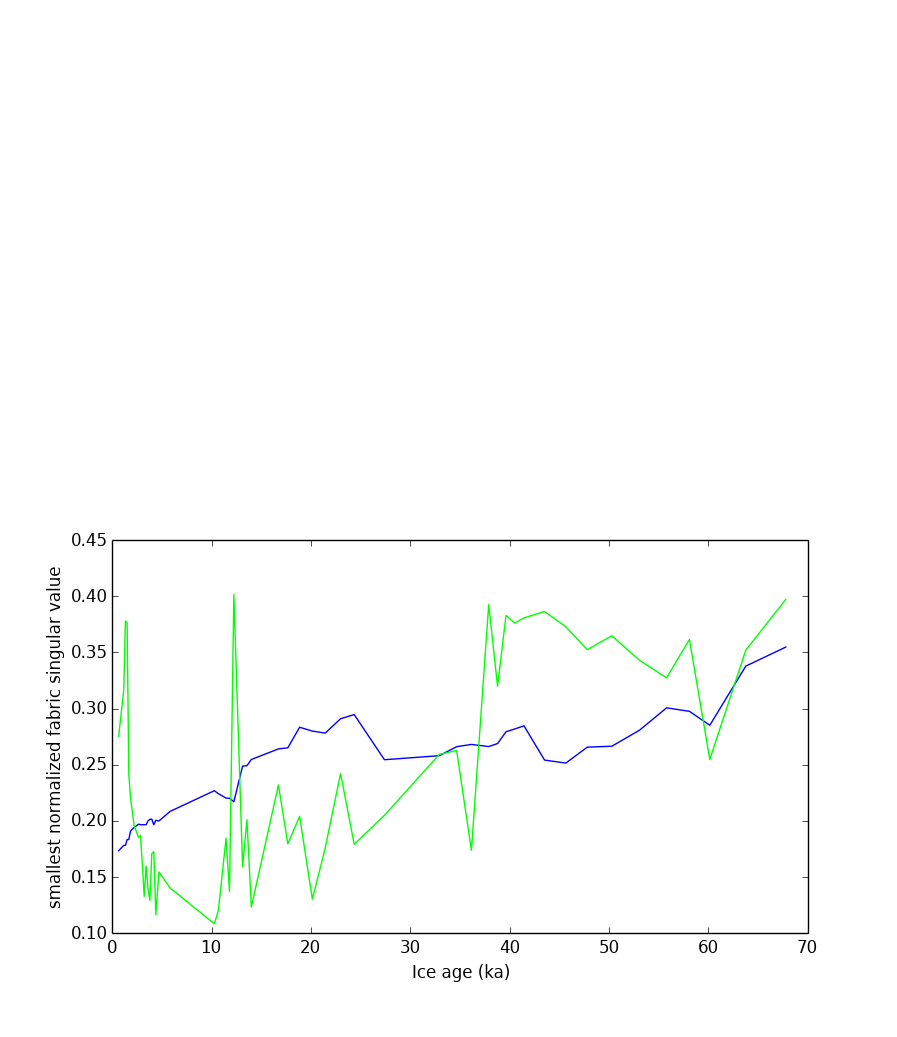
\includegraphics[width=10cm]{waisfit}
\end{figure}
\begin{figure}
\caption{Scmidt plot of girdle fabric produced under uniaxial compression. The grains rotate to the vertical axis. As they do, they are consumed by grains with lower strain energy.} 
\includegraphics[width=7cm]{girdle}
\end{figure}
\section{Goals}
\begin{itemize}
\item In the near term, reproduce general small-girdle fabrics by modeling rotation and migration recrystallization. This will show that the model is able to handle recrystallization in arbitrary strain environments.

\item Reproduce WAIS divide thin sections, especially the transition between vertical girdle to single maxima. This may be able to be explained by changing impurity concentrations affecting grain mobility or initial farbic.

\item When the flow model is developed, I will investigate the coupling of the fabric model and the flow. In addition to effects such as boudinage which depend on differing rheologies, it will also be possible to investigate effects due purely to the interdependence of flow and fabric. Recent results \citep{montgomery-smith2011} show that coupled Stokes-Jefferys equations modeling fiber suspensions can induce intiial perturbations in the orientation distribution function to grow significantly in short amounts of time.

\end{itemize}
\bibliographystyle{agu}
\bibliography{anis}
\end{document}
